\documentclass[11pt,letterpaper]{report}
\usepackage[latin1]{inputenc}
\usepackage{amsmath}
\usepackage{amsfonts}
\usepackage{amssymb}
\usepackage{graphicx}
\usepackage{color}
\usepackage{enumitem}
\usepackage[dvipsnames]{xcolor}
\definecolor{codegray}{gray}{0.9}
\newcommand{\code}[1]{\colorbox{codegray}{\texttt{#1}}}
\graphicspath{{./images/}{IR}}
%\newcommand{\LF}{}  % turn on to display large format
\ifdefined \LF
\usepackage[left=2.0cm, top=2.0cm, landscape]{geometry}  % for large format landscape
\else
\usepackage[left=2.0cm, top=2.0cm]{geometry}
\fi
\usepackage{fancyhdr}
\pagestyle{fancy}
\fancyhead{}
\lhead{CS333}
\chead{Project 1 Test Report}
\rhead{Alexander DuPree}
\begin{document}
\title{Project 1 Test Report}
\author{Alexander DuPree}

\ifdefined \LF
{\Large     % large print start
\fi

  \maketitle
  \section*{Introduction}
  \noindent
  The following test report documents the tests performed for project one. The test cases and strategies closely follow the project one rubric. 

  Each section contains test cases related to the sections topic. Each test case will describe the name of the test, 
  the expected result, actual result, as well as a discussion and indication of the Pass/Fail status. 
  The actual result will be provided in the form of a screen shot of the console. 

  \section*{System Call Tracing}
  This section presents all tests related to tracing system calls within the xv6 system. 
  Test cases follow closely those outlined in the rubric. \hfill \break
  
  \noindent\textbf{Test Case:} \emph{With PRINT\_SYSCALLS set to 0 in the Makefile}
  
  \noindent\textbf{Assertions:}
  \begin{enumerate}[]
  \item Code correctly compiles
  \item No trace information is displayed
  \end{enumerate}  
  
  \noindent\textbf{Status:} \textcolor{ForestGreen}{\textbf{PASS}}
  
  \begin{figure}[h!]
	\centering
	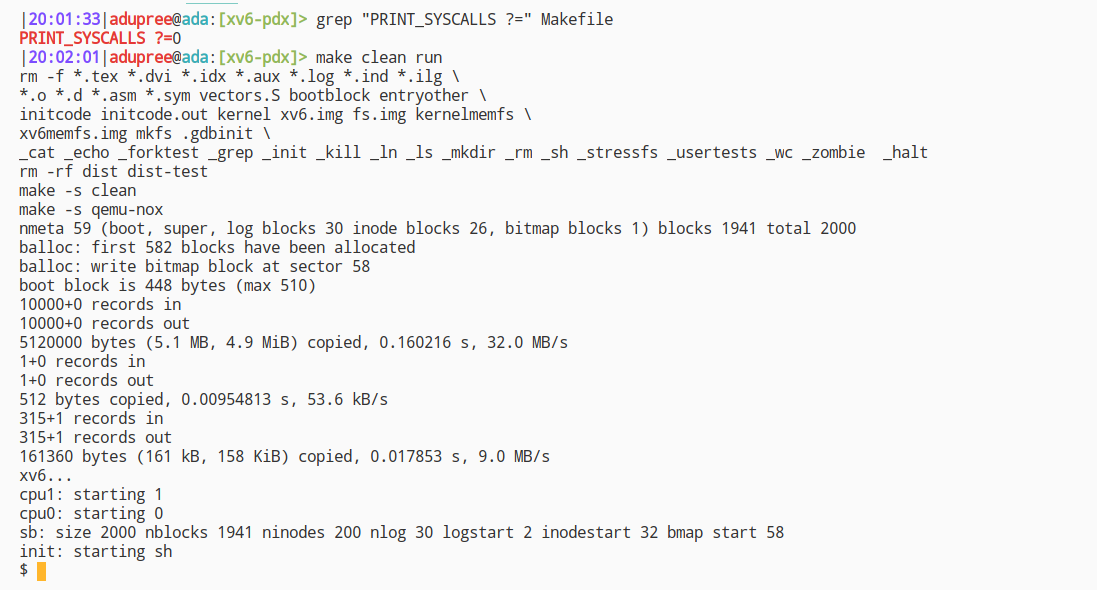
\includegraphics[width=1\linewidth]{test1.png}
	\caption[PRINT\_SYSCALLS=0]{Compilation and execution with PRINT\_SYSCALLS set to 0.}
	\label{fig:P1compileP0-1}
  \end{figure}

  The command \code{grep "PRINT\_SYSCALLS ?=" Makefile} shows that the PRINT\_SYSCALLS macro is indeed turned off.
  The following command \code{make clean run} demonstrates that the code correctly compiles and the output does not display any trace information.
  Furthermore, it should be noted that the timestamps for each command was performed within thirty seconds of each other.
  
\pagebreak

  \noindent\textbf{Test Case:} \emph{With PRINT\_SYSCALLS set to 1 in the Makefile}
  
  \noindent\textbf{Assertions:}
  \begin{enumerate}[]
  \item Code correctly compiles
  \item Trace information is displayed
  \item Correct call trace on boot
  \end{enumerate}  
  
  \noindent\textbf{Status:} \textcolor{ForestGreen}{\textbf{PASS}} \hfill \break
  
  \begin{figure}[h!]
	\centering
	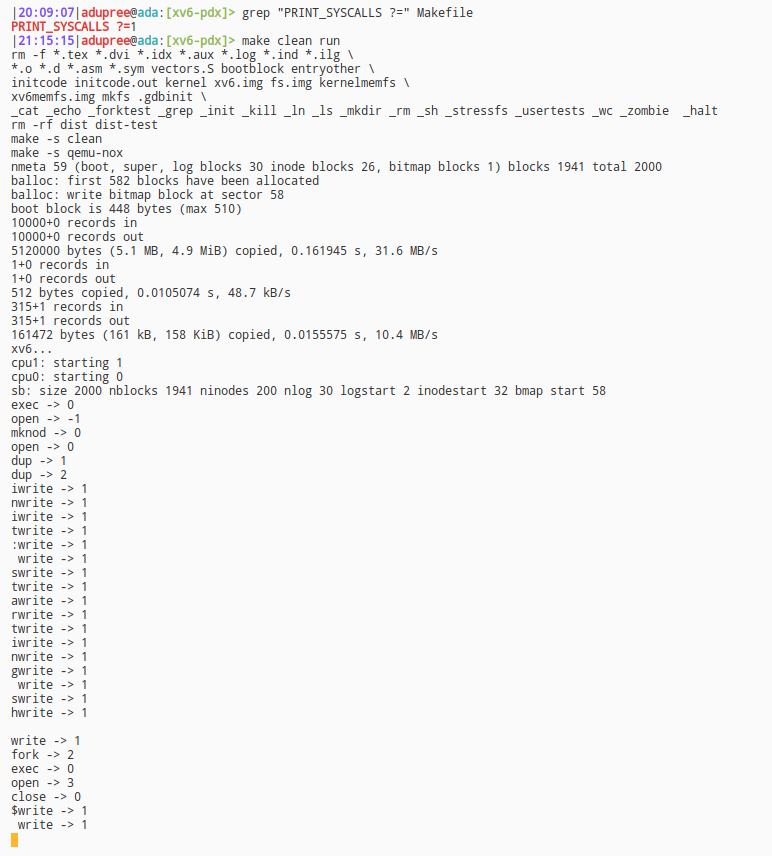
\includegraphics[height=\linewidth]{test2.png}
	\caption[PRINT\_SYSCALLS=0]{Compilation and Boot call trace with PRINT\_SYSCALLS set to 1.}
	\label{fig:P1compileP0-1}
  \end{figure}

  \pagebreak

  The command \code{grep "PRINT\_SYSCALLS ?=" Makefile} shows that the PRINT\_SYSCALLS macro is indeed turned on.
  The following command \code{make clean run} demonstrates that the code correctly compiles and the output displays
  trace information for the system calls. The system call trace in Figure 2 matches the trace in the project description, which means that this is the correct call trace on boot.
  Furthermore, it should be noted that the timestamps for each command was performed within 10 seconds of each other.

  \pagebreak

  \section*{Conditional Compilation and Date System Call}
  This section presents tests related to the conditional compilation of the CS333\_P1 project flag and the Date system call.
  Test cases follow closely those outlined in the rubric. \hfill \break
  
  \noindent\textbf{Test Case:} \emph{With CS333\_P1 turned off, when CS333\_PROJECT is set to 0}
  
  \noindent\textbf{Assertions:}
  \begin{enumerate}[]
  \item Code correctly compiles
  \item Kernel boots
  \item forktest runs to completion correctly
  \item usertests runs to completion correctly
  \end{enumerate}  
  
  \noindent\textbf{Status:} \textcolor{ForestGreen}{\textbf{PASS}}
  
  \begin{figure}[h!]
	\centering
	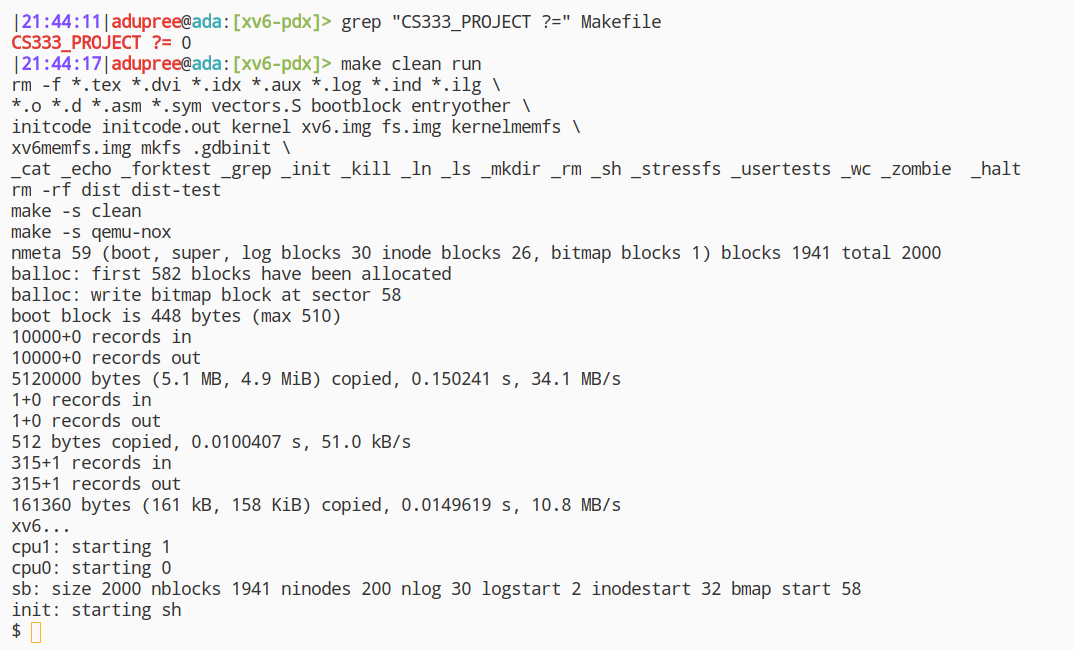
\includegraphics[width=1\linewidth]{test3.png}
	\caption[PRINT\_SYSCALLS=0]{Compilation and Kernel Boot with CS333\_P1 turned off.}
	\label{fig:P1compileP0-1}
  \end{figure}

  \begin{figure}[h!]
	\centering
	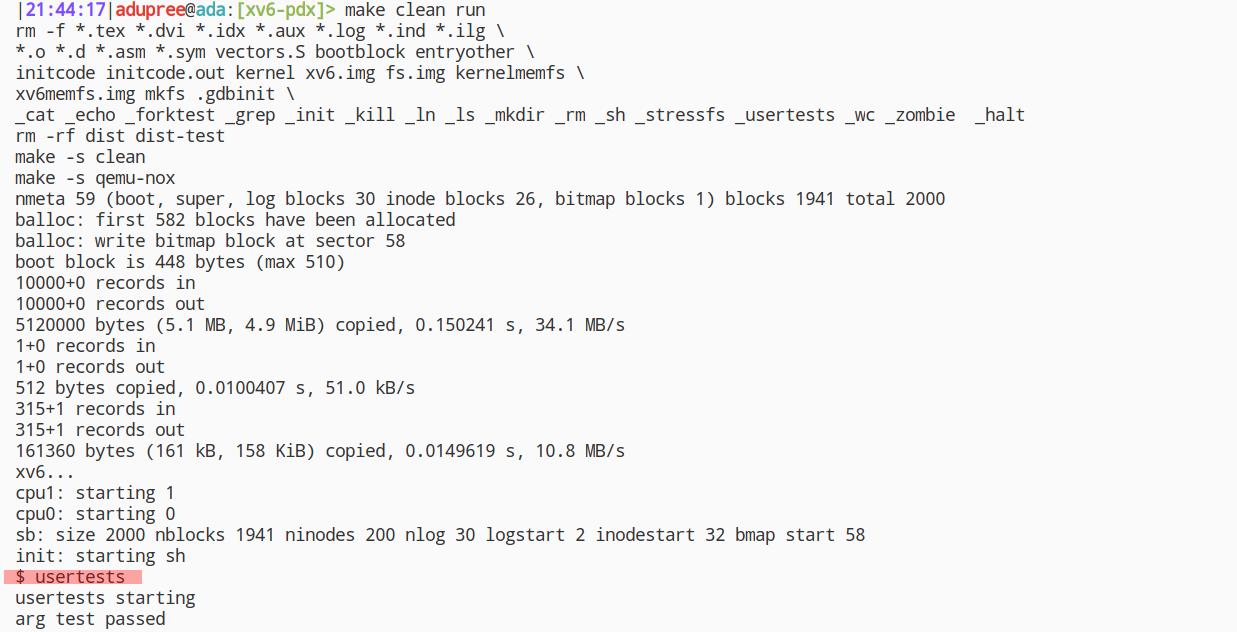
\includegraphics[width=1\linewidth]{test3-cont2.png}
	\caption[PRINT\_SYSCALLS=0]{Execution of usertests from the same session.}
	\label{fig:P1compileP0-1}
  \end{figure}

  \begin{figure}[h!]
	\centering
	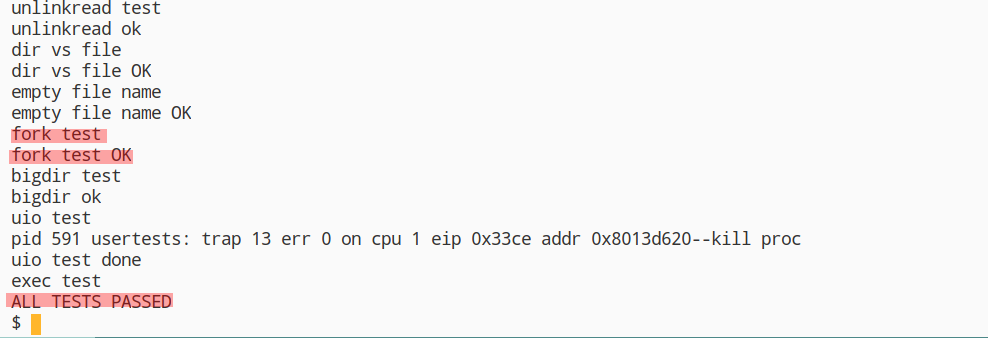
\includegraphics[width=1\linewidth]{test3-cont.png}
	\caption[PRINT\_SYSCALLS=0]{Results of usertests with output elided.}
	\label{fig:P1compileP0-1}
  \end{figure}
  
  Figure 3, 4, and 5 present the results of this test case. The command \code{grep "CS333\_PROJECT ?=" Makefile}
  shows that the CS333\_PROJECT is defined with 0. The following command \code{make clean run} demonstrates that 
  the code correctly compiles the kernel successfully boots. Because \code{forktest} is included with the \code{usertests}
  only the user tests were ran. The results of which are shown in figure 4 and 5. Due to the size of the test, much of the 
  output was elided. 
  
\pagebreak
  
  \noindent\textbf{Test Case:} \emph{With CS333\_P1 turned on, when CS333\_PROJECT is set to 1}
  
  \noindent\textbf{Assertions:}
  \begin{enumerate}[]
  \item Code correctly compiles
  \item Kernel boots
  \item forktest runs to completion correctly
  \item usertests runs to completion correctly
  \item The date command prints correct information
  \item The date command prints information in the correct format
  \end{enumerate}  
  
  \noindent\textbf{Status:} \textcolor{ForestGreen}{\textbf{PASS}}
  
  \begin{figure}[h!]
	\centering
	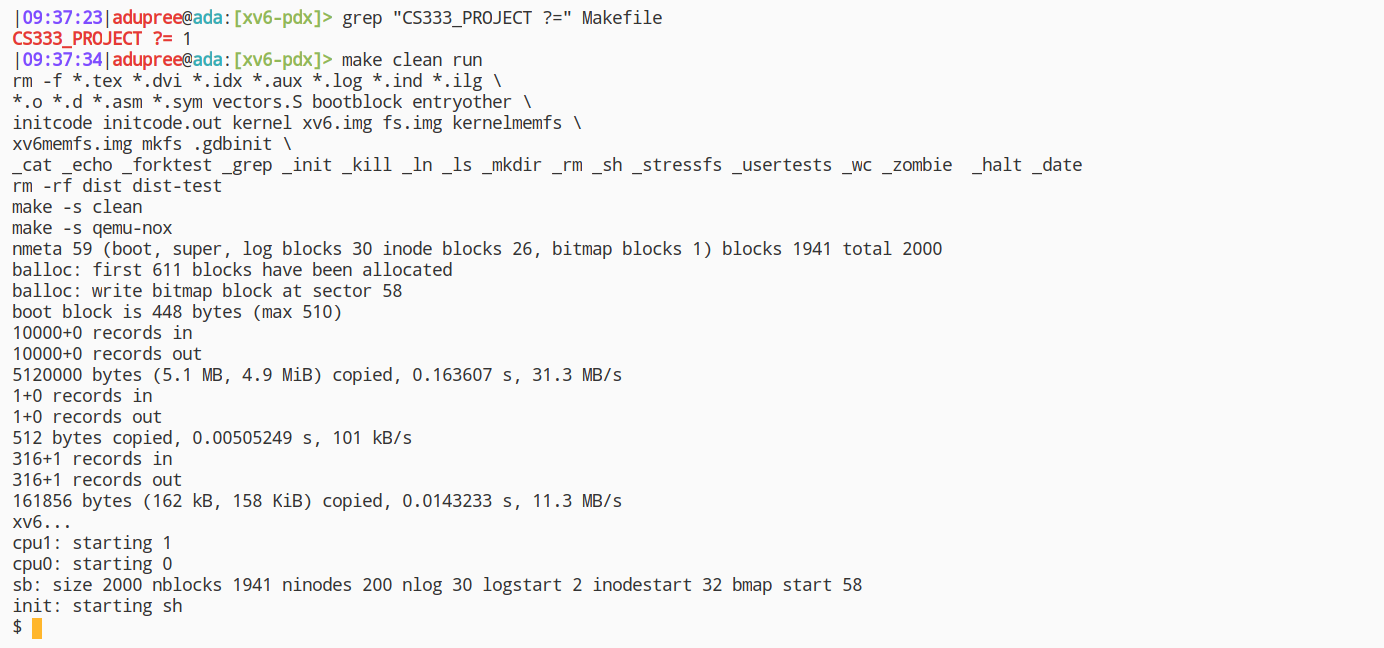
\includegraphics[width=1\linewidth]{test4.png}
	\caption[PRINT\_SYSCALLS=0]{Compilation and Kernel Boot with CS333\_P1 turned on.}
	\label{fig:P1compileP0-1}
  \end{figure}

  \begin{figure}[h!]
	\centering
	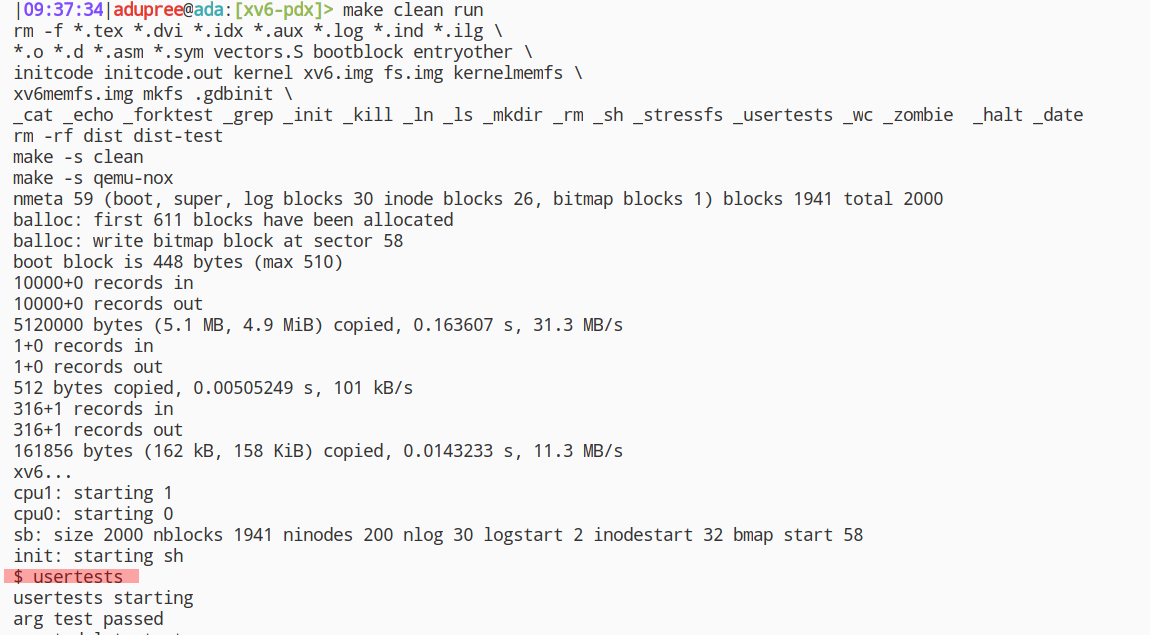
\includegraphics[width=1\linewidth]{test4-cont.png}
	\caption[PRINT\_SYSCALLS=0]{Execution of usertests from the same session with CS333\_P1 defined.}
	\label{fig:P1compileP0-1}
  \end{figure}

  \begin{figure}[h!]
	\centering
	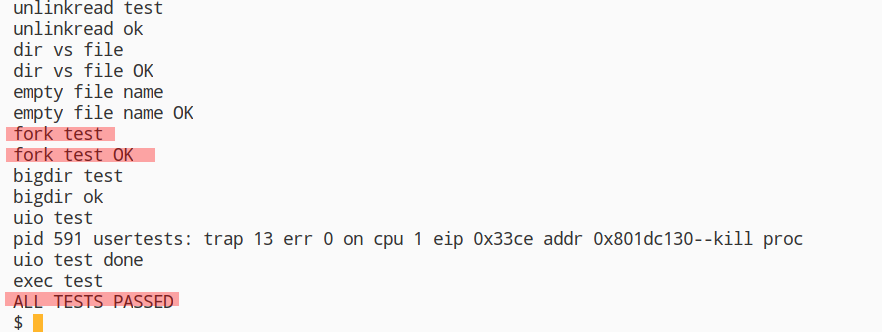
\includegraphics[width=1\linewidth]{test4-cont2.png}
	\caption[PRINT\_SYSCALLS=0]{Results of usertests with output elided and CS333\_P1 defined.}
	\label{fig:P1compileP0-1}
  \end{figure}

  \begin{figure}[h!]
	\centering
	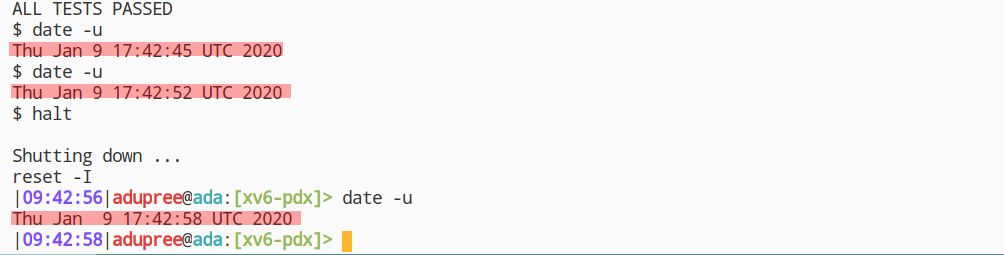
\includegraphics[width=1\linewidth]{test4-cont3.png}
	\caption[PRINT\_SYSCALLS=0]{Execution of date command, twice within xv6 and once on host machine.}
	\label{fig:P1compileP0-1}
  \end{figure}

\pagebreak

  Figures 6, 7, 8, and 9 present the results of this test case. In figure 6,
  the command 'grep "CS333\_PROJECT ?= Makefile' shows the the CS333\_PROJECT flag is set to 1.
  Following that is the command \code{make clean run} which demonstrates that the code correctly 
  compiles and the kernel boots successfully. Because \code{forktest} is included with 
  the \code{usertests}, only the user tests were ran, as illustrated in Figure 7. Figure 8 shows
  that all user tests pass. Figure 9 presents that the date system call is working correctly and 
  displays the correct information in the correct format. Note that the command \code{date -u} is 
  issued twice within the xv6 session to demonstrate that the date command provides different timestamps
  as expected. Also, the \code{date -u} is issued in the host machines terminal as well to prove 
  that the inormation and format is correct. Furthermore, the timestamps from each date call is 
  different and are done over a span of 15 seconds. 

\pagebreak

  \section*{Control-P}
  This section presents tests related to the Control-P console interrupt 
  and process information dump. Test cases follow closely those outlined in the 
  rubric. \hfill \break

  \noindent\textbf{Test Case:} \emph{Issuing control sequence 'Control-P' at runtime}
  
  \noindent\textbf{Assertions:}
  \begin{enumerate}[]
  \item Correct header displayed
  \item Output is aligned with header
  \item Correct and updated data is displayed
  \end{enumerate}  
  
  \noindent\textbf{Status:} \textcolor{ForestGreen}{\textbf{PASS}} \hfill \break
  
  \begin{figure}[h!]
	\centering
	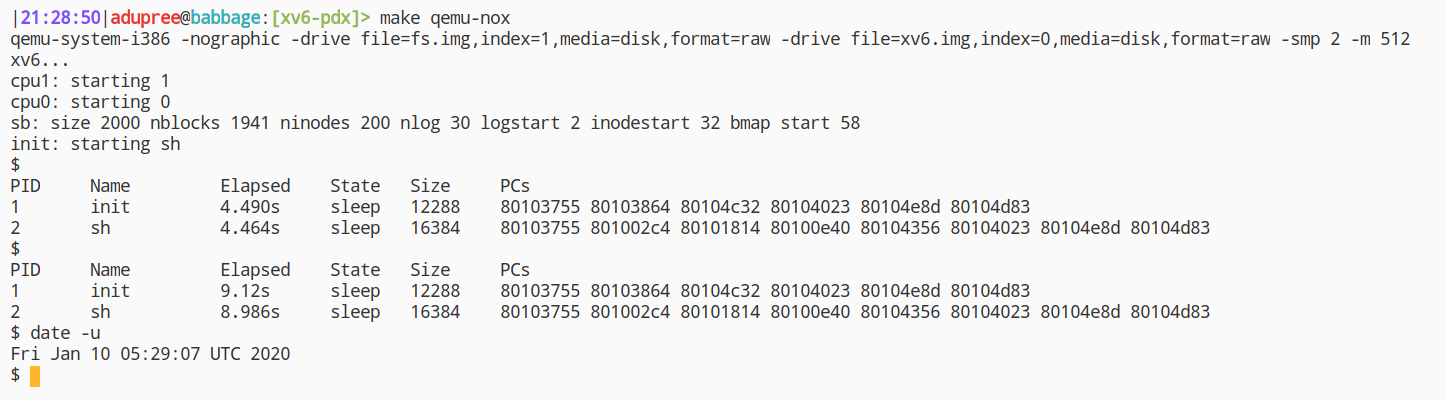
\includegraphics[width=\linewidth]{test5.png}
	\caption[PRINT\_SYSCALLS=0]{Compilation and Boot call trace with PRINT\_SYSCALLS set to 1.}
	\label{fig:P1compileP0-1}
  \end{figure}

  First, we can see that the header presented in Figure 10 displays the required fields
  outlined in the project description. The data displayed is aligned with the correct fields
  and is correct for the system. As expected, the init process is the oldest process, 
  and succesive uses of 'control-p' shows the elapsed time to be increasing for all processes. 


  \pagebreak

\ifdefined \LF
} % large print end
\fi

\end{document}